\section{はじめに}
自動運転における事故防止を目的とした障害物回避のた
めに障害物を認識し，自車から障害物までの距離を推定す
る必要がある．自動運転車でよく用いられる距離センサは
LiDAR(Light Detection and Ranging)である．しかし，
LiDAR は高価であり，メンテナンスに手間がかかる．そこ
で本研究では安価な単眼カメラによる障害物検出を目的と
する．

単眼カメラによる深度推定法として NDDepth\cite{1}や
MIMDepth\cite{2}などがある．しかし，これらの手法は単眼
カメラ画像のみで深度を推定するため，推定結果を実距離
にするスケールパラメータが不定であり，正確な距離を推
定することは困難である．以降，スケールが特定された深
度を距離，スケールが特定されていない深度を単に深度と
して区別して使用する．

単眼カメラ画像に加えて，自動運転用に作成された三次
元地図\reffig{3Dmap}を入力に用いることで，障害物までの距
離を推定できるPMOD-Net\cite{3}がある．正確な距離情報を
持つ三次元地図により，PMOD-Net は単眼カメラ画像で正
確な距離を推定しつつ障害物検出が可能である．

PMOD-Net は，三次元地図と単眼カメラ画像を入力とし
て，Semantic Segmentation と距離推定をマルチタスク
に行う．Semantic Segmentation で三次元地図上に存在
しない人や車などの動的障害物を検出することにより，距
離推定タスクで動的障害物の距離も推定可能にした．しか
し，三次元地図は動的障害物の距離情報を持たないため，
地図上に存在する障害物の距離推定精度に比べて，動的障
害物の距離推定精度は低い．そこで本研究は，単眼カメラ
を用いて，三次元地図上に存在しない動的障害物までの距
離を推定するという課題に取り組む．
\begin{figure}[t]
  \centering
  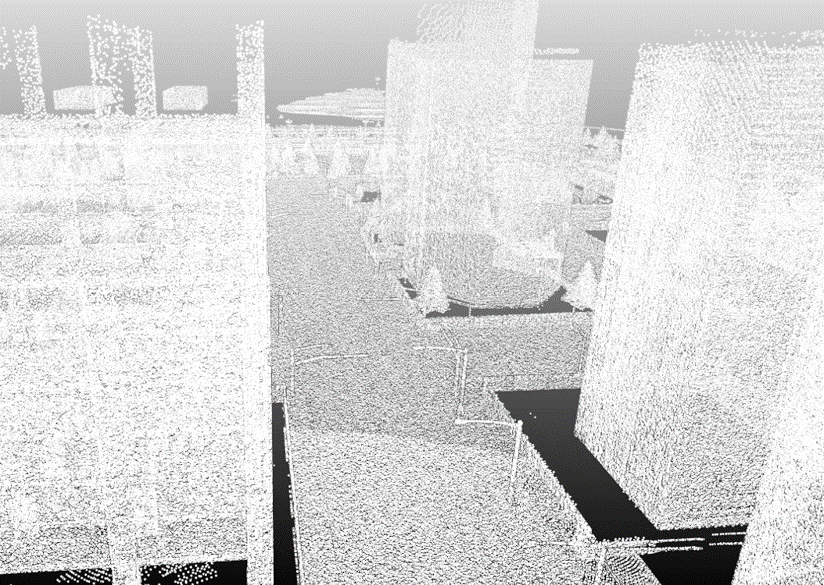
\includegraphics[width=0.95\linewidth]{img/intro/3Dmap.png}
  \caption{3D map}
  \label{3Dmap} 
\end{figure}

課題を解決するために，地図を使用する距離推定と地図
を使用しない深度推定の相補的な関係に着目した．三次元
地図を利用するPMOD-Net は距離を推定できるが，地図
の影響で動的障害物に対する距離推定精度は低い．地図を
使用しないNDDepth やMIMDepth は深度しか推定できないが，
動的障害物も含め，現在画像内にある全物体の相
対的な深度を精度よく推定できる．そこで，地図を使用し
ない単眼深度
推定法の出力を PMOD-Net へ入力する新手法 PMOD-
NetD（PMOD-Net with Depth）を開発する．三次元地
図という過去の距離情報と，単眼深度推定からの現在の深
度情報を統合し，単眼カメラによる高精度な障害物検出を
実現する．

本研究の学術的貢献は以下である．
\begin{enumerate}[1.]
  \begin{figure*}[t]
      \centering
      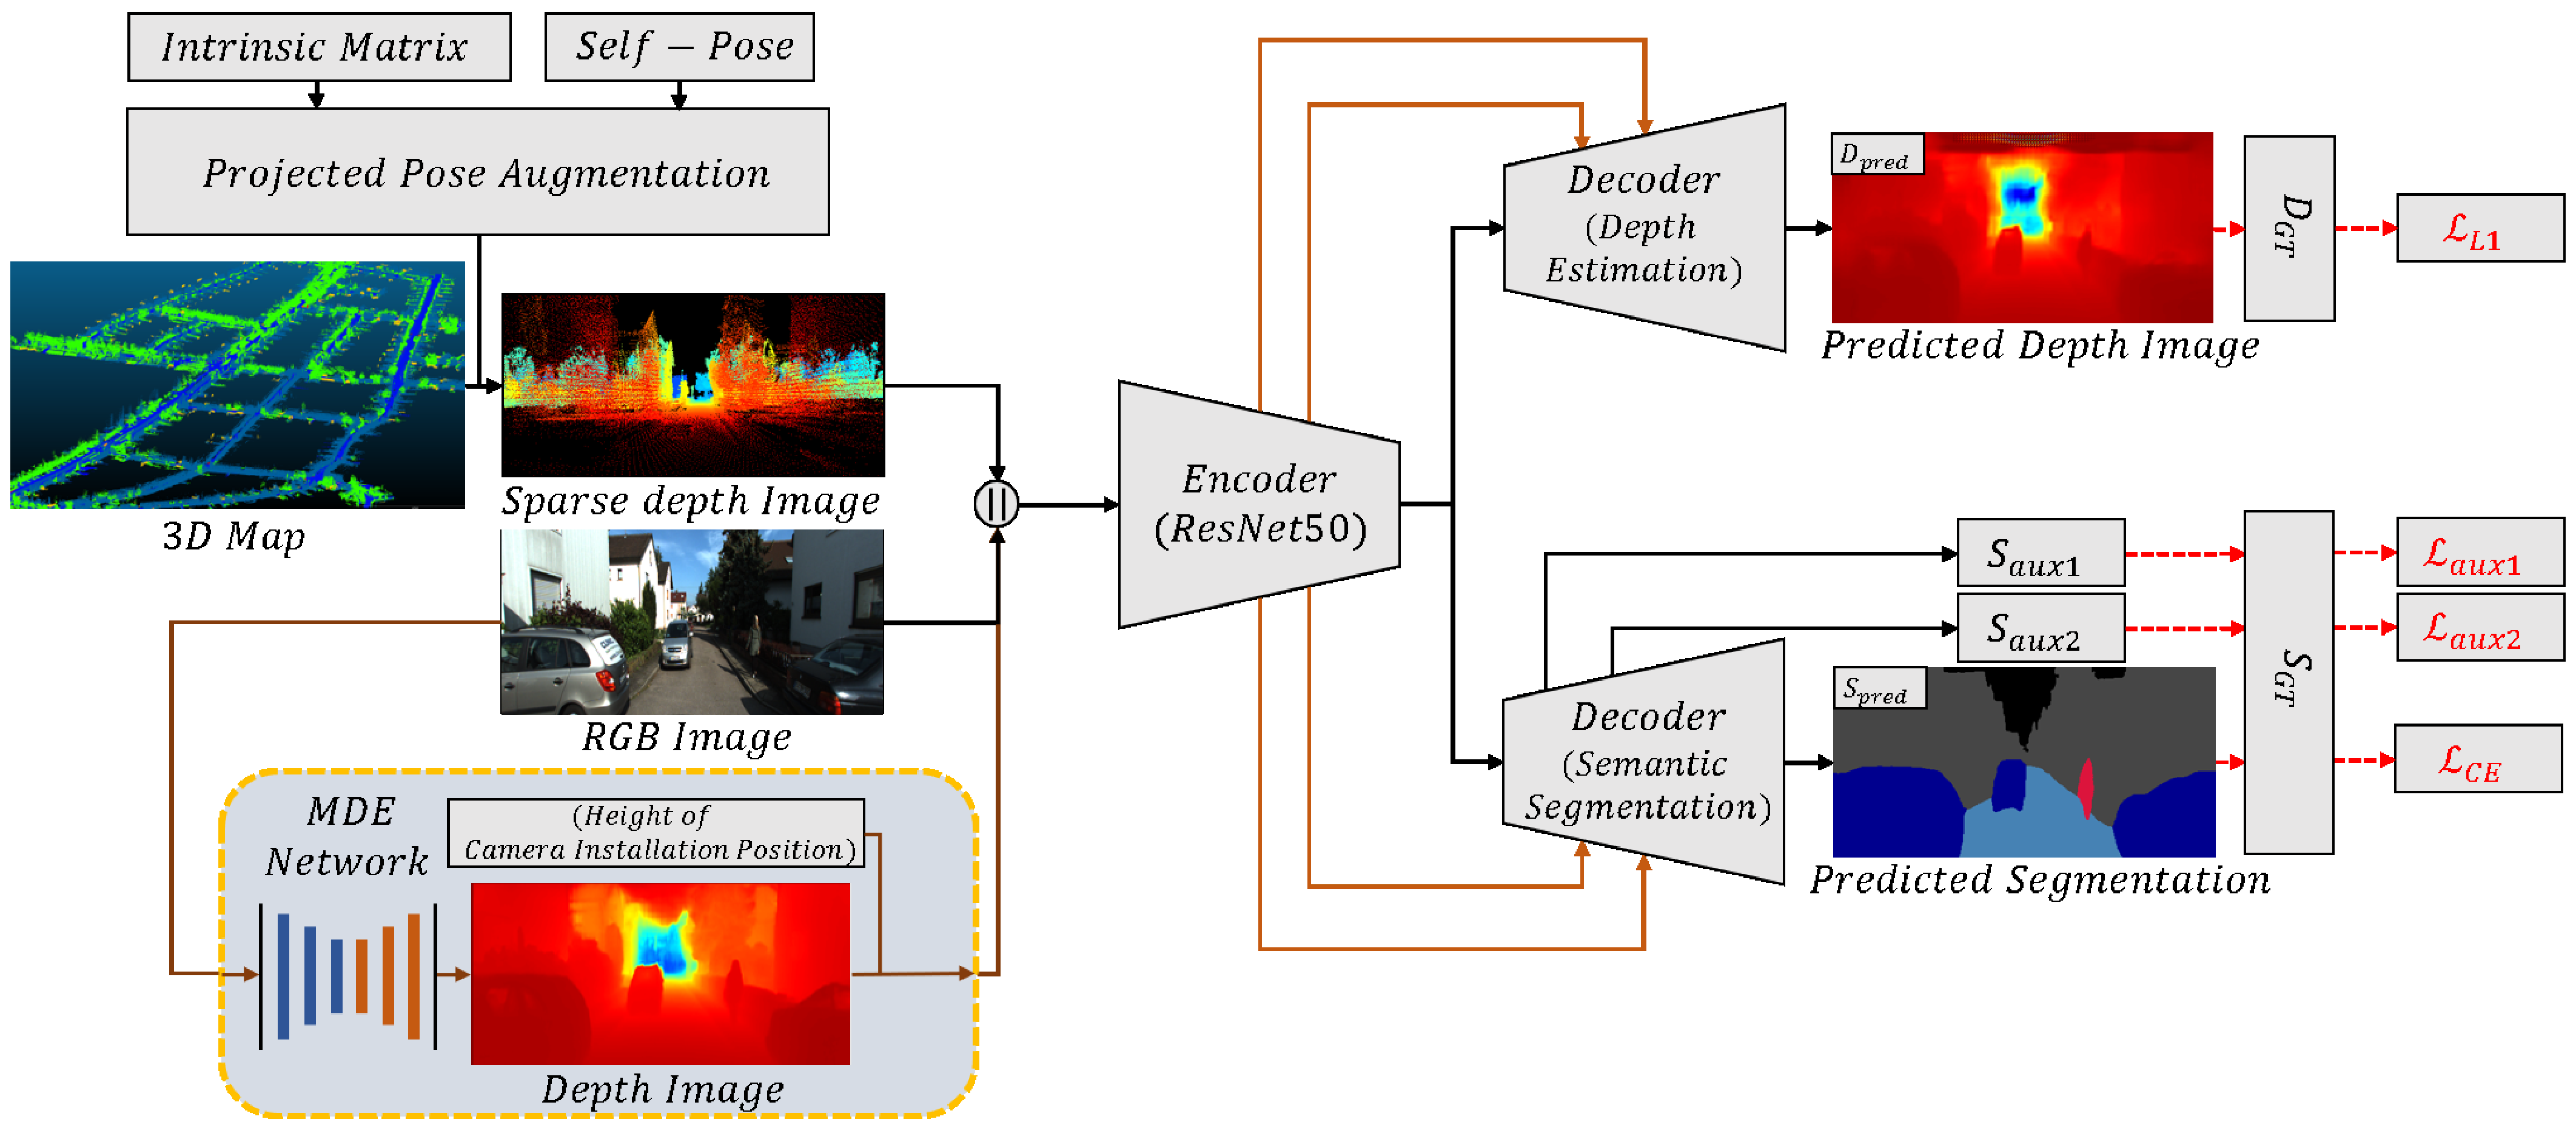
\includegraphics[width=0.95\linewidth]{img/method/network_architecture.eps}
      \caption{Network architecture of PMOD-NetD}
      \label{networkarchitecture} 
  \end{figure*}
  \item 三次元地図と単眼カメラを用いて三次元的に障害物検出を行う世界初のニューラルネットワークであるPMOD-Net を高精度化する新手法を開発した．
  \item スケールが不定であるため手法単体で扱うことが困難な単眼深度推定結果に対して三次元地図によるスケール調整が有効であることを示した．
  \item KITTI ベンチマークにおいて高順位の複数の単眼深度推定法に対して性能を高められることを確認し，手法を問わずに高精度化できる汎用性を示した．
\end{enumerate}